\section{Моделирование и его результаты}
	

	\subsection{Реализация модели}
	Модель (выражение \ref{eq:dls82e_model_S_p}) реализована на 
	языке программирования Python (версия 3.9.12) с применением 
	библиотеки TensorFlow (версия 2.8.0) и других библиотек	для научных
	вычислений.

	Модель частотного скана реализованна в виде отдельного класса \\
	\emph{FrequencyScan()} в модуле \emph{fsmodels.py}. Код 
	прокоментирован. Все параметры снабжены адекватными значениями по 
	умолчанию. В дальнейшем планируется дополнение документации и 
	перенос всех программных инструментов для обработки 
	экспериментальных данных в один пакет.

	Модель реализует две функции:
	\begin{enumerate}
		\item Вычисление частотного скана по заданным параметрам и 
		заданному вектору десятичных логарифмов частот опорной функции.
		\item Идентификация параметров модели частотного скана по 
		экспериментальным данным.
	\end{enumerate}
	Имеется возможность вывода значений параметров модели на каждой 
	итерации при идентификации. Примеры использования модели можно найти
	в файле \emph{tensorflow\_model.ipynb} (ПО Jupyter Notebook в составе 
	дистрибудтива Anaconda).

	Программа при каждом вычислении значения $\phi\left(\tau,F_0,
	t_1\right)$	(выражение \ref{eq:dls82e_model_phi}) находит 
	\(
		\max{\left[
	    \tau F_0 e^{-\frac{0.05}{\tau F_0}}
	    \left(1-e^{\frac{t_1 F_0-0.45}{\tau F_0}}
	    -e^{-\frac{0.5}{\tau F_0}}+
	    e^{\frac{t_1 F_0-0.95}{\tau F_0}}\right)
	    \right]}
    \)
	методом	градиентного спуска и вычисляет масштабный множитель $M$ 
	(выражение \ref{eq:dls82e_model_M}).

	Идентификация параметров модели производится методом градиетного 
	спуска, при этом минимизируется среднеквадратическая ошибка между 
	значениями, полученными в результате измерений, и результатами 
	моделирования (выражение \ref{eq:mse}).
	\begin{equation}
		\label{eq:mse}
		E = \frac{1}{n}\sum_{i=1}^{n}\left(y_i - y_i^*\right)^2,
	\end{equation}
	где
	\begin{description}
		\item[$y_i$] -- значения, полученные в результате измерений,
		\item[$y_i^*$] -- значения, полученные в результате моделирования,
		\item[$n$] -- количество измерений.
	\end{description}

	Градиентный спуск везде реализован с помощью библиотеки TensorFlow,
	которая использует алгоритм дифференцирования на графе вычислений,
	таким образом, производная берётся символьно (точно), затем вычисляется
	её значение, по этому точность вычисления градиента ограничена только
	разрядностью чисел \cite{hands_on_ml}.

	\textbf{Для ускорения процесса идентификации и улучшения сходимости
	в модели вместо постоянной времени сигнала релаксации $\tau$ 
	выполняется идентификация величины $\rho = log10(\tau)$. По этим же
	и некоторым	другим техническим причинам при вычислении частотного 
	скана на вход модели нужно подавать не вектор частот опорной 
	функции, а вектор их десятичных логарифмов.}

	На рисунке \ref{pic:identification_test} показан пример результата
	идентификации модели на тестовых (специально сгенерированных) данных.

	\begin{figure}[ht]
		\centering
		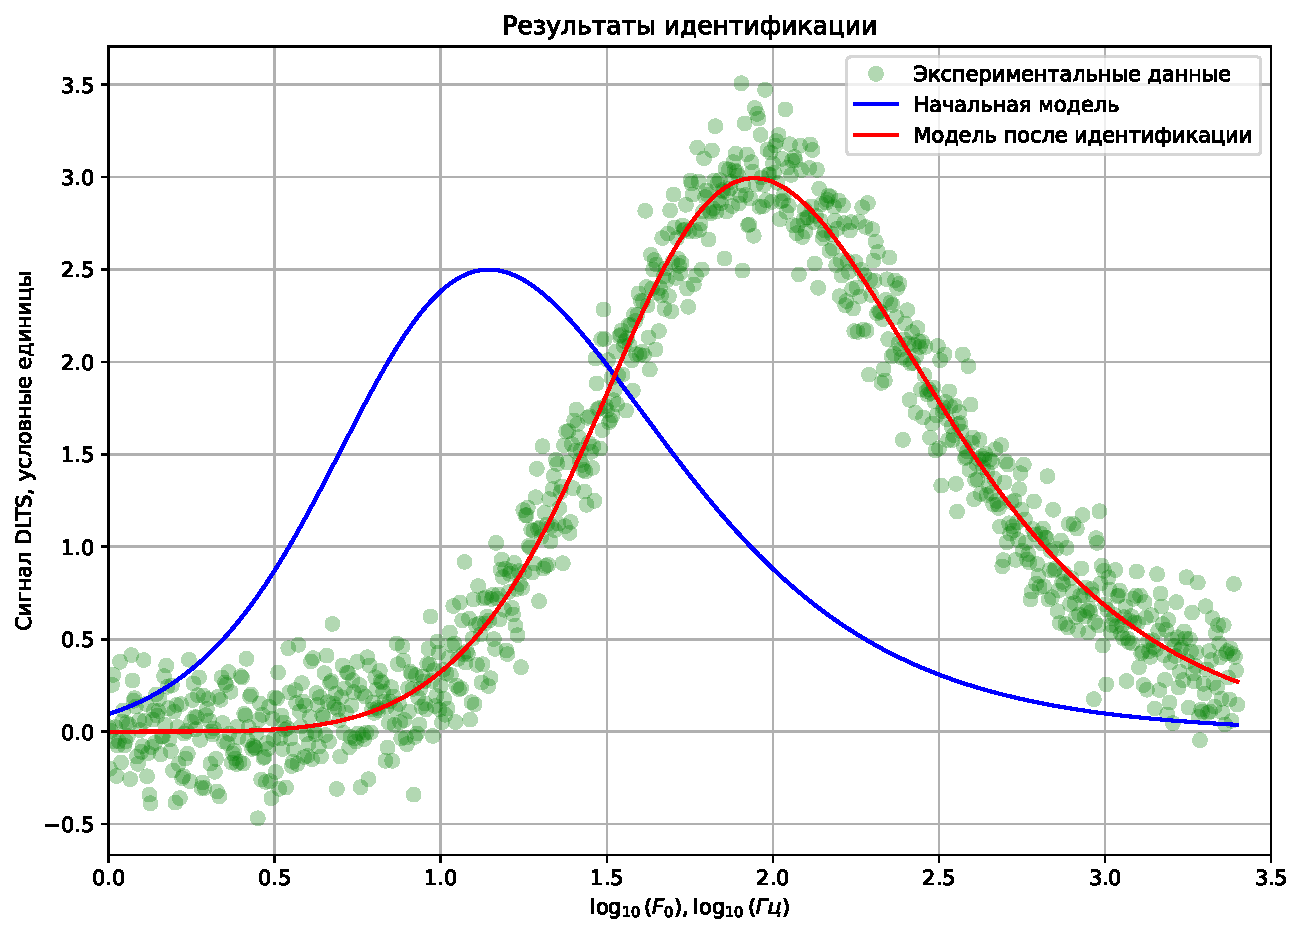
\includegraphics[width=0.75\textwidth]{identification_test}
		\caption{Пример результата идентификации модели.}
		\label{pic:identification_test}
	\end{figure}

	На рисунке \ref{pic:param_path} показан <<путь>> изменеия параметров 
	(постоянной времени и амплитуды) при идентификации. Красными точками 
	отмечены значения параметров на каждой итерации, изолинии показывают 
	значения среднеквадратической ошибки.

	\begin{figure}[ht]
		\centering
		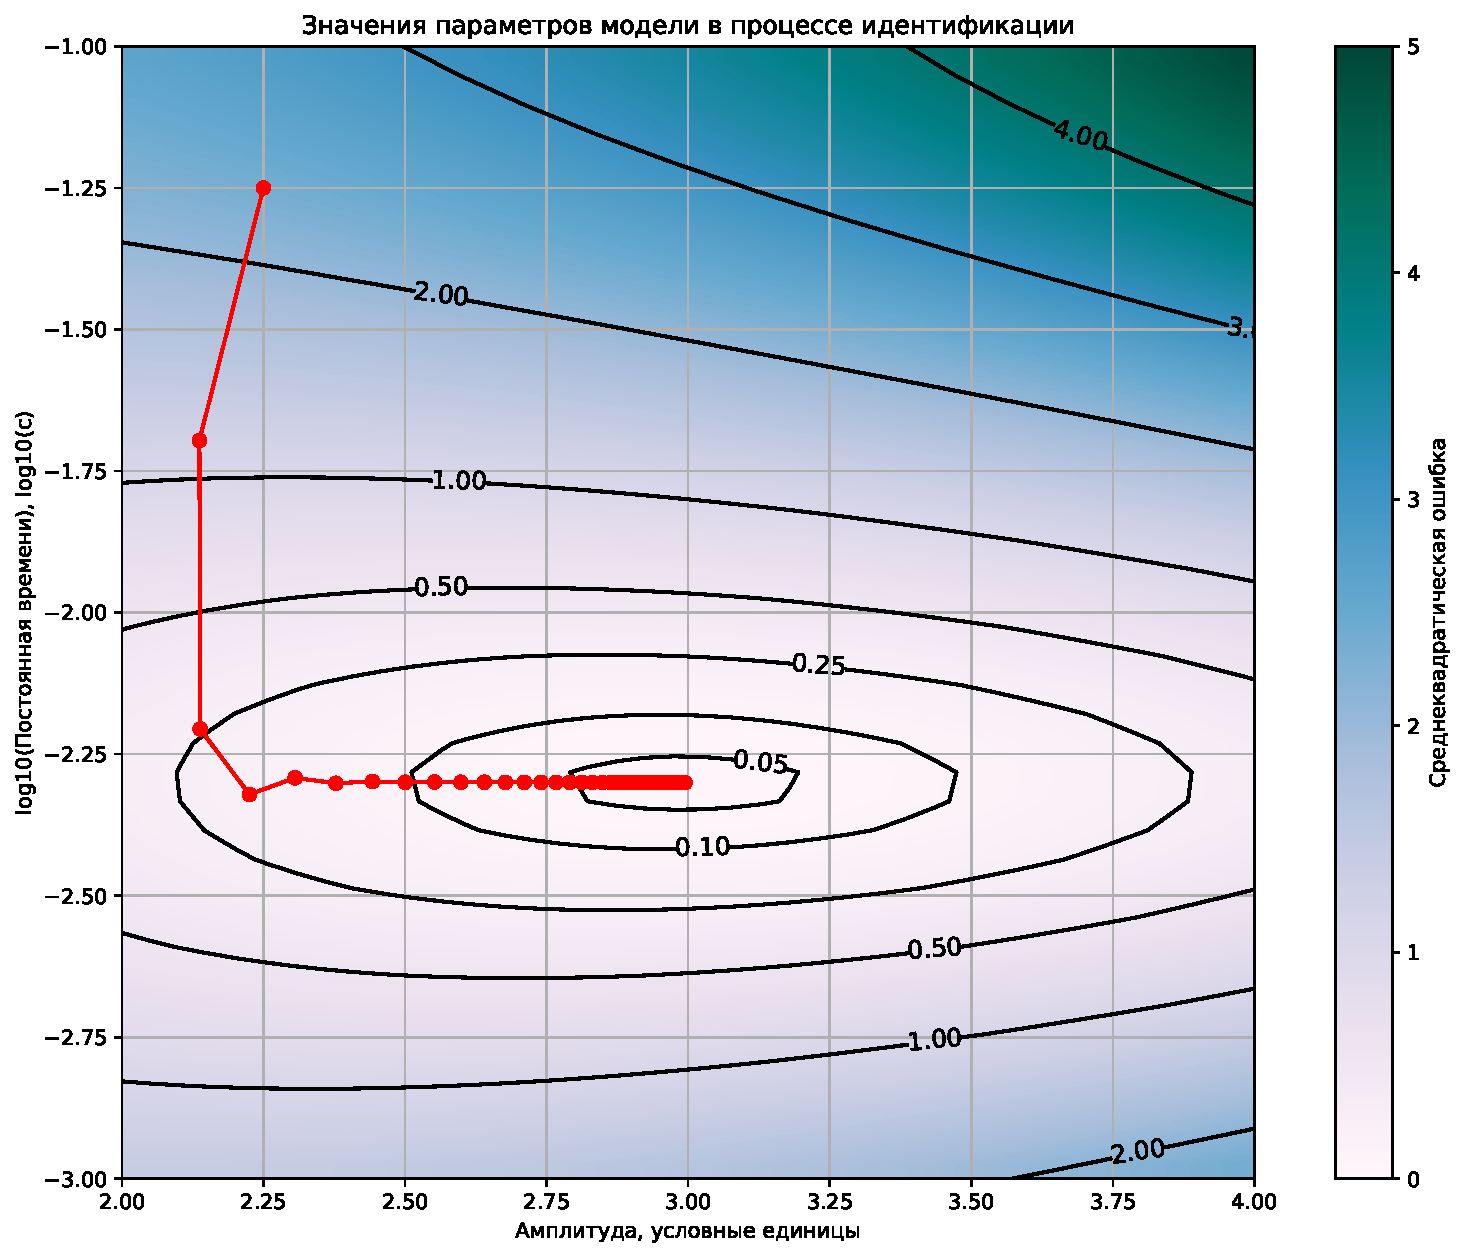
\includegraphics[width=\textwidth]{path}
		\caption{<<Путь>> изменеия параметров при идентификации.}
		\label{pic:param_path}
	\end{figure}


	\subsection{Результаты моделирования в отсутствии шума}

	\begin{table}[ht]
		\begin{tabular}{|l|l|l|l|l|l|l|l|l|l|l|}
            \hline
			\# & amplitude & time\_constant\_power & p\_coef & loss     & tc\_0  & tc\_1 & tc\_2   & amp\\ \hline
			0  & 3         & -2                    & 1       & 7.65E-10 & 0.01   & 0.01  & 0.01    & 1  \\ \hline
			1  & 3         & -2                    & 0.999   & 3.04E-08 & 0.0104 & 0.01  & 0.00962 & 1  \\ \hline
			2  & 3         & -2                    & 0.997   & 4.73E-07 & 0.0108 & 0.01  & 0.00926 & 1  \\ \hline
			3  & 2.99      & -2                    & 0.994   & 2.38E-06 & 0.0112 & 0.01  & 0.00891 & 1  \\ \hline
			4  & 2.98      & -2                    & 0.989   & 7.47E-06 & 0.0117 & 0.01  & 0.00858 & 1  \\ \hline
			5  & 2.97      & -2                    & 0.984   & 1.81E-05 & 0.0121 & 0.01  & 0.00825 & 1  \\ \hline
			6  & 2.96      & -2                    & 0.976   & 3.71E-05 & 0.0126 & 0.01  & 0.00794 & 1  \\ \hline
			7  & 2.95      & -2                    & 0.968   & 6.78E-05 & 0.0131 & 0.01  & 0.00764 & 1  \\ \hline
			8  & 2.93      & -2                    & 0.959   & 0.000114 & 0.0136 & 0.01  & 0.00736 & 1  \\ \hline
			9  & 2.92      & -2                    & 0.948   & 0.00018  & 0.0141 & 0.01  & 0.00708 & 1  \\ \hline
			10 & 2.9       & -2                    & 0.937   & 0.000269 & 0.0147 & 0.01  & 0.00681 & 1  \\ \hline
			11 & 2.88      & -2                    & 0.924   & 0.000386 & 0.0153 & 0.01  & 0.00656 & 1  \\ \hline
			12 & 2.85      & -2                    & 0.911   & 0.000535 & 0.0158 & 0.01  & 0.00631 & 1  \\ \hline
			13 & 2.83      & -2                    & 0.897   & 0.000719 & 0.0165 & 0.01  & 0.00607 & 1  \\ \hline
			14 & 2.81      & -2                    & 0.882   & 0.000943 & 0.0171 & 0.01  & 0.00584 & 1  \\ \hline
			15 & 2.78      & -2                    & 0.866   & 0.00121  & 0.0178 & 0.01  & 0.00562 & 1  \\ \hline
			16 & 2.75      & -2                    & 0.85    & 0.00152  & 0.0185 & 0.01  & 0.00541 & 1  \\ \hline
			17 & 2.72      & -2                    & 0.834   & 0.00188  & 0.0192 & 0.01  & 0.00521 & 1  \\ \hline
			18 & 2.69      & -2                    & 0.817   & 0.00229  & 0.02   & 0.01  & 0.00501 & 1  \\ \hline
			19 & 2.66      & -2                    & 0.799   & 0.00274  & 0.0207 & 0.01  & 0.00482 & 1  \\ \hline
			20 & 2.63      & -2                    & 0.781   & 0.00325  & 0.0215 & 0.01  & 0.00464 & 1  \\ \hline
			21 & 2.6       & -2                    & 0.763   & 0.00381  & 0.0224 & 0.01  & 0.00447 & 1  \\ \hline
			22 & 2.57      & -2                    & 0.745   & 0.00441  & 0.0233 & 0.01  & 0.0043  & 1  \\ \hline
			23 & 2.53      & -1.99                 & 0.727   & 0.00506  & 0.0242 & 0.01  & 0.00414 & 1  \\ \hline
			24 & 2.5       & -1.99                 & 0.708   & 0.00574  & 0.0251 & 0.01  & 0.00398 & 1  \\ \hline
			25 & 2.47      & -1.99                 & 0.69    & 0.00647  & 0.0261 & 0.01  & 0.00383 & 1  \\ \hline
			26 & 2.43      & -1.99                 & 0.671   & 0.00723  & 0.0271 & 0.01  & 0.00369 & 1  \\ \hline
			27 & 2.4       & -1.99                 & 0.653   & 0.00803  & 0.0282 & 0.01  & 0.00355 & 1  \\ \hline
			28 & 2.36      & -1.99                 & 0.635   & 0.00884  & 0.0293 & 0.01  & 0.00341 & 1  \\ \hline
			29 & 2.33      & -1.99                 & 0.616   & 0.00968  & 0.0304 & 0.01  & 0.00329 & 1  \\ \hline
			30 & 2.29      & -1.98                 & 0.598   & 0.0105   & 0.0316 & 0.01  & 0.00316 & 1  \\ \hline
		\end{tabular}
	\end{table}